\documentclass[a4paper,12pt]{report}


\usepackage[paper=A4,pagesize]{typearea}
\usepackage{afterpage}
\usepackage{siunitx}
\usepackage{url}
\usepackage{graphicx}
\usepackage{pdflscape}
\usepackage{lmodern,textcomp}
\usepackage{longtable}
\usepackage{adjustbox}
\usepackage{pdflscape}
\usepackage[square,numbers]{natbib}
\usepackage{notoccite}
\usepackage{chapterbib, tabularx}
\usepackage{booktabs}
\usepackage{multirow}
\usepackage{tabularx}
\usepackage[euler]{textgreek}
\usepackage[center]{caption}
\usepackage{acronym}
\usepackage{xr}
\usepackage{float}
\DeclareUnicodeCharacter{2005}{ }
\DeclareUnicodeCharacter{2606}{ }
\DeclareUnicodeCharacter{2212}{ }
\DeclareUnicodeCharacter{E5F8}{ }


\newcolumntype{C}[1]{>{\centering\arraybackslash}p{#1}}

\externaldocument[lit-]{Chapter2/ch2}
\externaldocument[exp-]{Experimental/ch1}
\externaldocument[dft-]{Chapter3/ch3}
\externaldocument[proc-]{Chapter4/ch4}



\newcolumntype{L}{>{\centering\arraybackslash}m{3cm}}

\begin{document}

\title{Developing a hydrogen impurity enrichment device for measuring impurities in fuel-grade hydrogen}
\author{Marc Plunkett}
\date{\today}
\maketitle

\chapter*{Declaration of Originality}
I hereby declare that the work reported in this thesis was composed and originated entirely by me. Information derived from published and unpublished results of others has been acknowledged in the text and in the relevant references included within the thesis.

\noindent\newline
\textbf{Marc Plunkett}\newline

\includegraphics[width=50mm,scale=0.5]{figures/sig.png}\newline

\noindent
Imperial College London\newline

The copyright of this thesis rests with the author and is made available under a 'Creative Commons Attribution Non-Commercial No Derivatives' licence. Researchers are free to copy, distribute or transmit the thesis on the condition that they attribute it, that they do not use it for commercial purposes and that they do not alter, transform or build upon it. For any reuse or redistribution, researchers must make clear to others the licence terms of this work.


\chapter*{Executive summary}
The copyright of this thesis rests with the author and is made available under a 'Creative Commons Attribution Non-Commercial No Derivatives' licence. Researchers are free to copy, distribute or transmit the thesis on the condition that they attribute it, that they do not use it for commercial purposes and that they do not alter, transform or build upon it. For any reuse or redistribution, researchers must make clear to others the licence terms of this work.

The copyright of this thesis rests with the author and is made available under a 'Creative Commons Attribution Non-Commercial No Derivatives' licence. Researchers are free to copy, distribute or transmit the thesis on the condition that they attribute it, that they do not use it for commercial purposes and that they do not alter, transform or build upon it. For any reuse or redistribution, researchers must make clear to others the licence terms of this work.

The copyright of this thesis rests with the author and is made available under a 'Creative Commons Attribution Non-Commercial No Derivatives' licence. Researchers are free to copy, distribute or transmit the thesis on the condition that they attribute it, that they do not use it for commercial purposes and that they do not alter, transform or build upon it. For any reuse or redistribution, researchers must make clear to others the licence terms of this work.

The copyright of this thesis rests with the author and is made available under a 'Creative Commons Attribution Non-Commercial No Derivatives' licence. Researchers are free to copy, distribute or transmit the thesis on the condition that they attribute it, that they do not use it for commercial purposes and that they do not alter, transform or build upon it. For any reuse or redistribution, researchers must make clear to others the licence terms of this work.

The copyright of this thesis rests with the author and is made available under a 'Creative Commons Attribution Non-Commercial No Derivatives' licence. Researchers are free to copy, distribute or transmit the thesis on the condition that they attribute it, that they do not use it for commercial purposes and that they do not alter, transform or build upon it. For any reuse or redistribution, researchers must make clear to others the licence terms of this work.

The copyright of this thesis rests with the author and is made available under a 'Creative Commons Attribution Non-Commercial No Derivatives' licence. Researchers are free to copy, distribute or.


\chapter*{Acknowledgements}
Throughout the writing of this dissertation I have received a great deal of support and assistance. I  would  first  like  to  thank  my  supervisor,  Dr.  M.  Gellar,  whose  expertise  was  invaluable  in  the formulating of the research topic and methodology in particular.

I would like to acknowledge my colleagues from my internship at Central P. for their wonderful collaboration. You supported me greatly and were always willing to help me. I would particularly like to single out my supervisor at Central P., Ms. P. Buffay. Phoebe, I want to thank you for your excellent  cooperation  and  for  all  of  the  opportunities  I  was  given  to  conduct  my  research  and further my dissertation at Central P.

I would also like to thank my tutors, Messrs. R. Geller and C. Bing, for their valuable guidance. You  provided  me  with  the  tools  that  I  needed  to  choose  the  right  direction  and  successfully complete my dissertation.

In addition, I would like to thank my parents for their wise counsel and sympathetic ear. You are always there for me. Finally, there are my friends, who were of great support in deliberating over our problems and findings, as well as providing happy distraction to rest my mind outside of my research. 

\chapter*{List of Publications and Presentations}

\section*{Publications}
\begin{enumerate}
    \item \textbf{M. Plunkett}, K.Li, A. Murugan; Review of membrane technologies for hydrogen impurity enrichment; International Journal of Hydrogen Energy, 163 (2016), pp. F3119-F3124, 10.1149/2.0141611jes
    \item \textbf{M. Plunkett}, K.Li, A. Murugan; Review of membrane technologies for hydrogen impurity enrichment; International Journal of Hydrogen Energy, 163 (2016), pp. F3119-F3124, 10.1149/2.0141611jes
    \item \textbf{M. Plunkett}, K.Li, A. Murugan; Review of membrane technologies for hydrogen impurity enrichment; International Journal of Hydrogen Energy, 163 (2016), pp. F3119-F3124, 10.1149/2.0141611jes

\end{enumerate}

\section*{Oral Presentations}
\begin{enumerate}
    \item \textbf{M. Plunkett}, A. Murugan, K. Li; A hydrogen impurity enrichment device using Pd-Alloy membranes to support the hydrogen economy. Presented at International Conference for Membrane and Electromembrane Processes 2018, 13th – 16th May 2018, Prague, Czech Republic.
    \item \textbf{M. Plunkett}, A. Murugan, K. Li; A hydrogen impurity enrichment device using Pd-Alloy membranes to support the hydrogen economy. Presented at 15th International Conference on Inorganic Membranes, 18th – 22nd June 2018, Dresden, Germany. 
    \item \textbf{M. Plunkett}; The use of hydrogen selective materials for quality assurance of fuel grade hydrogen to ISO 14687-2 . Presented at 2nd bi-annual Gas and Particle Metrology symposium, 14th August, 2018, Teddington, United Kingdom 
\end{enumerate}

\listoffigures
\listoftables

\chapter*{List of Acronyms, Abbreviations and Symbols}
\begin{acronym}
    \acro{AHF}{Asymmetric Hollow Fibre}
    \acro{ATR}{Autothermal Reforming}
    \acro{ASTM}{American Society for Testing and Materials}
    \acro{BCC}{Body Centered Cubic}
    \acro{CEF}{Calculated Enrichment Factor}
    \acro{CRDS}{Cavity Ring Down Spectroscopy}
    \acro{CTE}{Coefficient of thermal expansion}
    \acro{CVD}{Chemical Vapour Deposition}
    \acro{DFT}{Density Functional Theory}
    \acro{DIN}{Deutsches Institut für Normung}
    \acro{EDS}{Energy-dispersive X-ray spectroscopy}
    \acro{EDP}{Electroplating Deposition}
    \acro{ELP}{Electroless Plating}
    \acro{EU}{European Union}
    \acro{FCC}{Face-centred cubic}
    \acro{FCEV}{Fuel Cell Electric Vehicle}
    \acro{FTIR}{Fourier-transform infrared spectroscopy}
    \acro{GC}{Gas Chromatography}
    \acro{GGA}{Generalized Gradient Approximation}
    \acro{GUI}{Graphical User Interface}
    \acro{HCP}{Hexagonal close packed}
    \acro{HEMS}{Hydrogen Elimination Mass Spectrometry}
    \acro{HIED}{Hydrogen Impurity Enrichment Device}
    \acro{HF}{Hollow Fibre}    
    \acro{HPC}{High-performance computing}
    \acro{HRS}{Hydrogen Refuelling Station}
    \acro{IEA}{International Energy Agency}
    \acro{ISO}{International Standards Orgainsation}
    \acro{kWh}{Kilo watt hour}
    \acro{LDA}{Local Density Approximation}
    \acro{LOHC}{Liquid Organic Hydrogen Carrier}
    \acro{MEA}{Membrane Electrode Assembly}
    \acro{MS}{Mass Spectrometry}
    \acro{NPL}{National Physical Laboratory}
    \acro{NPT}{National Pipe Thread}
    \acro{PDHID}{Pulsed discharge helium ionization detector}
    \acro{PEMFC}{Proten Exchange Membrane Fuel Cell}
    \acro{PID}{Proportional–integral–derivative}
    \acro{PPB}{Parts-Per-Billion}
    \acro{PPM}{Parts-Per-Million}
    \acro{PSA}{Pressure Swing Adsorption}
    \acro{PSS}{Porous Stainless Steel}
    \acro{PVD}{Physical Vapour Deposition}
    \acro{QE}{Quantum Espresso}
    \acro{SCD}{Sulfur chemiluminescence detector}
    \acro{SEM}{Scanning Electron Microscopy}
    \acro{SMR}{Steam Methane Reforming}
    \acro{UK}{United Kingdom}
    \acro{VOC}{Volatile Organic Compound}
    \acro{WGS}{Water Gas Shift}
    \acro{XRD}{X-ray diffraction}
    \acro{XPS}{X-ray photoerlectron spectroscopy}
    \acro{YSZ}{Ytrrium stabilized zirconium}

\end{acronym} 

\begin{acronym}
    \acro{Ag}{Silver}
    \acro{Ar}{Argon}
    \acro{Au}{Gold}
    \acro{CH4}[CH\textsubscript{4}]{Methane}
    \acro{Cu}{Copper}
    \acro{CO}{Carbon Monoxide}
    \acro{CO2}[CO\textsubscript{2}]{Carbon Dioxide}
    \acro{He}{Helium}
    \acro{H2}[H\textsubscript{2}]{Hydrogen}
    \acro{HCHO}{Formaldehyde}
    \acro{HCOOH}{Formic Acid}
    \acro{H2O}[H\textsubscript{2}O]{Water}
    \acro{N2H4}[N\textsubscript{2}H\textsubscript{4}]{Hydrazine}
    \acro{HCl}{Hydrochloric Acid}
    \acro{H2S}[H\textsubscript{2}S]{Hydrogen Sulphide}
    \acro{NaOH}{Ammonium hydroxide}
    \acro{Pd}{Palladium}
    \acro{PdNH34Cl2H2O}[PdNH\textsubscript{3}4Cl\textsubscript{2}H\textsubscript{2}O]{Tetra-amminepalladium (II) chloride monohydrate}
    \acro{SnCl2}[SnCl\textsubscript{2}]{Tin(ii)Chloride}
    \acro{Zn}{Zinc}

\end{acronym}


\tableofcontents


\chapter{Introduction}
\section{Problem statement}
Due to the damaging environmental effects of using fossil fuels in the transport sector, national and 
international targets have been set in order to reduce global CO\textsubscript{2} emissions.
In the UK for example, there is a plan to completely ban the sale of new conventional petroleum vehicles 
by as early as 2040. 
\cite{DepartmentforEnvironment2017} 
One proposed solution is further adoption of fuel cells and other energy generation methods which utilize
hydrogen as a carbon free energy source. 

Despite the fact that the technology for hydrogen powered fuel vehicles has existed since the early 1960’s, their application has been limited to providing power for space missions and other niche applications. It wasn’t until the late 90’s when developments in lowering the platinum catalyst loading and breakthroughs in the production of thin film electrodes drove the cost of fuel cells down to a level where they were a commercially viable option. As of 2017, a number of auto mobile manufacturers including Toyota,\cite{Toyota2015} Hyundai, \cite{Hyundai2015} Honda \cite{Honda} and Daimler \cite{Mohrdieck2014} now offer hydrogen vehicles commercially. It is also possible to retrofit a petroleum vehicle to run off hydrogen.\cite{FCell2016} Many countries both in the EU, and globally have ambitious hydrogen infrastructure plans over the next 10 years. This is in an effort to become less reliant on importing fossil fuels, increase their energy security, and transition to a carbon free energy system.

The development of the hydrogen economy is still in its infancy,  however several countries are aiming to deploy sizable hydrogen fuelling infrastructures over the next few decades. National reports state that Europe’s position in 2030 will be: UK - 1,100 hydrogen refuelling stations and 1.6 million fuel cell vehicles \cite{UKH2Mobility2013} France – 600 hydrogen refuelling stations and 0.8 million fuel cell vehicles \cite{Summerton2015}, Germany – 1,180 hydrogen refuelling stations \cite{Hayter2014} and 1.8 million fuel cell vehicles  and the Netherlands – 200 hydrogen refuelling stations and 0.2 million fuel cell vehicles. \cite{Hayter2014} The fuel cell system in a hydrogen vehicle can easily degrade if even parts-per-billion to parts-per-million level of some impurities are present in the hydrogen. Therefore, it is imperative that hydrogen purity, and techniques for verifying purity, are adequate to ensure customers vehicles are not inadvertently damaged by fluctuations in hydrogen composition. 

International standards advise that all hydrogen suppliers should prove that their product is pure enough to prevent degradation of fuel cell components. ISO 14687-2:2012 \cite{InternationalStandardISO14687-2:20122012}, shown in Table \ref{tab:1} specifies the maximum impurity levels of 13 impurities that are permissible in fuel cell hydrogen. ISO 14687-2:2012 includes some challenging hydrogen purity specifications mainly due to the impurity limits being below the limits of detection of the standard techniques commonly used to measure the concentration of these compounds. 

\begin{table}[]
    \caption{Concentration limits for ISO-14687 impurities}
    \centering
    \begin{tabular}{@{}cc@{}}
    \toprule
    \textbf{Characteristics}                  & \textbf{Regulation}    \\ \midrule
    Minimum mole fraction of hydrogen         & 99.97\%                \\
    Total non-hydrogen gases                  & 300 µmol mol-1         \\ \midrule
    \multicolumn{2}{c}{\textbf{Maximum concentration of individual components}} \\ \midrule
    Total Hydrocarbons (Methane basis)        & 5 µmol mol-1           \\
    Water                                     & 2 µmol mol-1           \\
    Oxygen                                    & 5 µmol mol-1           \\
    Helium                                    & 300 µmol mol-1         \\
    Carbon dioxide                            & 2 µmol mol-1           \\
    Carbon monoxide                           & 0.2 µmol mol-1         \\
    Total sulphur compounds (H\textsubscript{2}S basis)       & 0.004 µmol mol-1       \\
    Formaldehyde                              & 0.01 µmol mol-1        \\
    Formic acid                               & 0.2 µmol mol-1         \\
    Ammonia                                   & 0.1 µmol mol-1         \\
    Total halogenated compounds               & 0.05 µmol mol-1        \\
    Maximum particulate concentration         & 1 mg/kg                \\ \bottomrule
    \end{tabular}
    \label{tab:1}
\end{table}

Existing hydrogen purity laboratories are unable to perform traceable analysis to ISO 14687 
specifications because appropriate methods and standards have not been developed. The consequence 
of this is that hydrogen suppliers cannot provide evidence that their fuel meets these specifications and therefore are not permitted to supply hydrogen. Of the 13 gaseous impurities listed in 
ISO 14687-2, there is no single method for measuring all impurities. Laboratories must therefore use 
several instruments to perform such an analysis.  In 2015 Murugan et al published a review of methods 
for analysing the purity of fuel grade hydrogen \cite{Murugan2015}. They concluded that in order for a single laboratory to provide full hydrogen analysis to ISO 14687-2 specifications it would require 
a number of instruments including GCs, FTIR and CRDS. The capital cost of purchasing the gas 
analysers to perform analysis on the measurable impurities in a hydrogen sample can amount to 
>€500,000 \cite{Murugan2015} and hence performing analysis would be out of reach for many of the smaller 
laboratories. 

While the impurities listed in ISO 14687-2 are specified at extremely low amount fractions, 
many can be analysed at higher amount fractions through the use of cheap and routine gas 
analysers such as a GC-MS. Therefore a solution is to increase the concentration of impurities
above the limit of detection of a cheaper, more widespread analyser. These techniques are referred 
to as enrichment or pre-concentration. The most commonly used technique for pre-concentration 
of hydrogen fuel samples is referred to as ‘Hydrogen Impurity Enrichment’. This method involves 
passing the sample through a semi permeable membrane material, such as palladium, which only allows the passage of hydrogen.\cite{NathanW.Ockwig2007a} As hydrogen leaves the system, the impurities remain, increasing in concentration with time as more hydrogen permeates through the membrane. This increase in concentration is referred to as the enrichment factor and once the enrichment is complete the sample can then be analysed at these higher concentrations, and using the enrichment factor, the original composition of the sample can be found. 

The accuracy, cost and time taken for a hydrogen enrichment device is highly defpendent on the membrane material. Different materials will allow hydrogen to permeate at different rates and will interact differently with impurities that may be present in hydrogen.\cite{NathanW.Ockwig2007a} While hydrogen enrichment is a promising technology for hydrogen impurity measurement, more research must be done to properly understand how different membrane materials interact with common hydrogen impurities, and therefore identify the most appropriate material.

\section{Research Objectives}
This thesis will focus on developing hydrogen impurity enrichment as a low-cost technique for measuring 
the impurities in fuel grade hydrogen to ISO 14687-2 specification. 
This study will revolve around the membrane materials used to concentrate the impurities in hydrogen samples 
and will aim to determine the best material, and conditions for the hydrogen impurity enrichment device. 
The thesis aims are as follows:
\begin{itemize}
\item Identify the best material for enriching impurities based on the degree of interaction and reactivity with the impurities shown in Table 1 
\item Finalise a protocol for national measurement institutions to follow when enriching a hydrogen sample. 
\item Convert the experimental set up in to a commercially viable prototype which could be used in analytical laboratories
\item Perform full enrichment using these three conclusions on a real sample taken from a hydrogen refuelling station
\end{itemize}
In order to determine suitable enrichment material ‘Density Functional Theory (DFT) will be used to screen a number of materials for their suitability as an impurity enrichment membrane on their simulated 
interaction strength with ISO 14687 impurities. 

The best performing membrane materials simulated in Chapter 3 will then be synthesised in Chapter 4. 
The hydrogen permeability of each material under a number of ISO 14687-2 impurities will be measured to 
validate the simulation results and further narrow down the most suitable membrane composition. 
Following from this the best membrane will be used in Chapter 5 which will describe the design and 
commercialisation of the final hydrogen impurity enrichment device. The design of the enrichment device 
will include an uncertainty budget of the technique, automation of the device, and compliance to European standards.

Finally the new device, featuring the most suitable membrane, redesigned process, and protocols for tracer enrichment will be tested using a real sample taken from a hydrogen refuelling station.

\section{Thesis structure and presentation}
This thesis consists of 7 chapters, which includes the ‘Introduction’, ‘Literature Review’, 
experimental chapters and ‘Conclusion’. The thesis structure is visualised in figure \ref{funnel}. 
The experimental chapters address different aspects of development of hydrogen metrology techniques as 
described above. 

\begin{figure}[H]
  \includegraphics[width=\linewidth]{figures/funnel.png}
  \caption{Schematic presentation of the thesis structure}
  \label{funnel}
\end{figure}


\renewcommand{\bibname}{References}
\bibliographystyle{unsrtnat}
\bibliography{library.bib}

\chapter{Literature review}

\section{Hydrogen impurity enrichment}
'Hydrogen impurity enrichment' is a term for any technique which involves increasing the 
concentration of impurities within a hydrogen sample by means of removing the hydrogen matrix gas. 
There are two previous reports of impurity enrichment being used as a technique for hydrogen impurity 
analysis. 
The first report by Papadis et al at Argonne National Laboratory used a Pd/Cu \cite{Ahmed2010}
coated Pd/Ag membrane for non-sulphur containing hydrogen samples and a Pd/Au coated Pd/Ag membrane for sulphur 
containing hydrogen samples to enrich impurities in a 50 bar sample. 
The analyte gas used contained 
N\textsubscript{2}, CH\textsubscript{4} and CO\textsubscript{2} at 100 \textmu mol/mol and an additional 
 2 \textmu mol/mol of H\textsubscript{2}S during sulphur tests sulphur. 
The enrichment was calculated by using measured values of temperature and pressure along with the 
non-ideal gas law, this was represented through a 'calculated enrichment factor' as shown in equations \ref{eq:1}
and \ref{eq:2}. 

\begin{equation} \label{eq:1}
    % \frac{(\frac{P_{1,a} V_1)}{Z_{1,a} RT_{1,a}})}
    CEF_{NI} = \frac{\frac{P_{1,a} V_1}{Z_{1,a}RT_{1,a}}\frac{P_{2,a} V_2}{Z_{2,a}RT_{2,a}}-\frac{P_{1,b} V_1}{Z_{1,b}RT_{1,b}}}{\frac{P_{2,b} V_2}{Z_{2,b}RT_{2,b}}}
\end{equation}

\begin{equation}\label{eq:2}
    y_{i,a} = \frac{y_{i,b}}{CEF}
\end{equation}
The set-up was able to reach enrichment factors of around 32 for non-sulphur tests and 15 
for sulphur tests. The non-sulphur tests closely matched with the actual component concentrations, 
however in the second set of tests there was some loss of sulphur observed, most likely due to the 
formation of palladium sulphide on the surface of the membrane, or through wall catalysed reactions. 

\renewcommand{\bibname}{References}
\bibliographystyle{unsrtnat}
\bibliography{library.bib}

\chapter{Experimental methods}

\section{Simulations}
Density functional theory calculations were performed using the Quantum Espresso (QE) ab 
initio simulation package using the generalized gradient approximation with the PW91 
functional to describe electron-correlation effects. Ion-electron interactions were described 
using ultra-soft pseudopotentials. A plane-wave expansion with a cut-off of 233.73 eV was used 
in all calculations. Geometry relaxations were performed with a conjugate gradient method until 
the forces on all unconstrained atoms were less than 0.03 eV/A. A Monkhorst Pack mesh with 
4x4x4 k-points was used for all calculations.

The supercell used contained 20 metal atoms and one gaseous molecule located on one of four 
available sites on the metal lattice. It was assumed that all palladium systems adopt the 
substitutional; random fcc structure. Metal atoms were randomly distributed among the fcc 
lattice in the supercell. All atoms were allowed to relax during the calculation, with the 
volume of the super cell fixed at the optimised volume of the super cell without adsorbed 
molecules. 

Geometry optimization was performed to get the lattice constant and total energy of each 
alloy prior to adsorption of gaseous molecules. 

\section{Membrane manufacture}

\subsection{Materials used}
\subsection{Support fabritcation}
The YSZ 3\% hollow fibre substrates with a desired micro-structure were fabricated by a 
fingering induced phase-inversion process, followed by high temperature sintering. A uniform 
ceramic suspension, with 60 wt.\% solid loading, was prepared by ball milling. After degassing, 
the ceramic suspension was transferred into 200 mL stainless steel syringes and extruded 
through a tube-in-orifice spinneret (outer diameter 3 mm, inner diameter 1.2 mm) into a 
coagulation bath with no air gap. An extrusion rate of 7 and 5 mL min-1 was adopted for 
ceramic suspension and bore fluid (15 wt.\% 1,4- dioxane in n-hexane), respectively. The formed 
precursor fibres were kept in deionized water for a minimum of 12 h, in order to remove the 
excessive solvent. After being gently washed with deionized water, the precursor fibres were 
dried at room temperature and sintered at 1400\textdegree C in a tubular furnace (Elite, Model TSH 
17/75/450).
\subsection{Membrane deposition}
\subsubsection{Electoless Plating}
Palladium silver, copper, gold, and ternary alloy compositions (expect for PdCuZr) were 
deposited onto the surface of the porous YSZ substrate through electroless plating. 
The process was performed in two steps; the first involves ‘activating’ the surface of the 
material intended for deposition by seeding the surface with particles of a metal with a 
higher electro positivity than the metal intended to be plated. Normally palladium is used due 
to its high electro positivity compared to other metals commonly plated through electroless 
deposition. This activation step is required for non-conductive supports such as ceramics and 
glass but may not be required for conductive supports depending on the specific support 
material and intended plating layer. The ‘activation’ step is followed by the ‘plating’ step 
where a solution containing a metallic salt, complexing agent, and stabilising agent is 
reduced through the use of a reducing agent, causing solid metal to be displaced from the 
solution, and due to the catalytic activity of the seeds placed in the prior step, forming a 
dense metal layer on the intended surface. Electroless plating results in a strongly adhered, 
dense metallic layer which can be deposited easily on a large range of morphologies.

Prior to deposition, the outer surface of the fibre was cleaned by sequential washings with a 
1:1 mixture of ethanol and water for 10 min in an ultrasonic bath, and were then dried overnight 
at 120\textdegree C.

Preceding electroless plating, the substrates were coated at one end with a gas tight glaze 
and sintered at 900\textdegree C for 1 hour. Prior to deposition, the outer surface of the fibre was 
cleaned by sequential washings with a 1:1 mixture of ethanol and water for 10 min in an 
ultrasonic bath, and were then dried overnight at 120 °C.

The substrates were then activated with Pd nuclei via sensitisation in an acidic SnCl2 
solution, followed by activation in an acidic PdCl2 solution. The sensitisation/activation 
process was carried out by immersing the glazed hollow fibre substrates sequentially in five 
chemical baths, i.e. acidic SnCl2 solution for 5 min; deionised water for 5 min, acidic PdCl2 
solution for 5 min; 0.01 M HCl solution for 2 min; and finally deionised water for 3 mins. 
All chemical baths were homogenised by stirring. The sensitisation/activation process was 
repeated for 6 cycles. The composition of each bath is shown in Table 2.

The substrates were then immersed in a Pd electroless plating (ELP) solution, at 60\textdegree C, 
in order to deposit metallic Pd layers onto the activated surface. The Pd ELP solution was 
prepared according to the composition presented in Table 2 and left to stabilize for 1 h in an 
ultrasonic bath prior to use. The volume of Pd ELP solution was fixed at 4 mL per cm2 of 
substrate surface area. The electroless plating procedure was performed twice, with a total 
plating time of 60 mins.

After the palladium coating the membranes were then subjected to one, or multiple, other 
plating steps of silver, gold, or copper. The plating time for silver was 30 minutes for one 
cycle and the volume of plating solution to substrate was the same as the palladium steps.

It should be noted that the deposition of gold is through immersion plating rather than 
electroless plating. Immersion plating is the process of applying adhering layers of nobler 
metals to another metal's surface by dipping the material in a heated nobler metal solution 
ion to produce a replacement reaction. This causes the deposition of a metallic coating on a 
base metal from solutions that contain coating metal. One metal is typically displaced by 
metal ions that have lower levels of oxidation potential, relative to the metal ion being 
displaced. The plating time for gold was 3 hours and the volume of plating solution to 
substrate was 4mL per cm3.

The resulting composite membranes consisting of multiple metal layers stacked were then heat 
treated at 500oC under an environment containing 25\% H2 in Ar balance for 24 hours in order 
to alloy the layers into a homogenous metal membrane.

\subsection{Materials testing}

\section{Membrane testing}
\subsection{Preparation of gas standards}
\subsection{Membrane testing rig}

\section{Hydrogen impurity enrichment}
\subsection{Device design}

\renewcommand{\bibname}{References}
\bibliographystyle{unsrtnat}
\bibliography{library.bib}

\chapter{Density functional theory as a screening method for dense metal membranes}

\section{Abstract}

\section{Introduction}
High impurity resistant dense metal membranes are being developed for hydrogen impurity enrichments of HRS samples with hydrogen derived from biomass, hydrocarbon or electrolysis. Metal membranes operate by selectively dissociating hydrogen, which then allows the hydrogen atoms to solubilize and subsequently permeate through the bulk of the separation layer. The problem is that many hydrogen impurities are also capable of adsorbing onto and interacting with the surface of many of the metals which comprise dense metal membranes. The impact of this adsorption can vary depending the molecule, Carbon monoxide for example will simply adsorb onto the surface and result in competitive adsorption between the hydrogen and impurity. Sulphur containing impurities which are commonly found in hydrocarbon sources and therefore are potentially present in any hydrogen produced from these methods. Sulphur containing impurities present more of a problem since they can potentially react with many metals used for hydrogen separation membranes. The impact of these contaminants can be minimized by designing alloy compositions that have a weaker attraction to the membrane, and therefore will have less of an affect at higher temperatures where these membranes operate.

Physically testing each potential membrane composition would be time consuming and costly due to the high price of palladium, the time required to synthesise specific membrane compositions, and performing the tests. Simulations provide a solution to this, allowing potential alloys to be screened for their interaction strength with each individual ISO 14687-2 impurity quickly, avoiding the cost of manufacturing each alliy composition. 

This chapter will calculate the behaviour of 14 palladium alloy composition under 13 ISO 14687-2 impurities. This is done by comparing the total energy of different configurations after relaxation of internal forces in the system. The close packed surfaces of palladium alloys were simulated as 

\section{Results and discussion}


\begin{table}[]
    \centering
    \caption{Simulated total energy values of ISO 14687-2 impurities}
    \label{gases}
    \begin{tabular}{@{}cc@{}}
    \toprule
    Gas          & \begin{tabular}[c]{@{}c@{}}Total Energy\\ $(kJ \times 10^{-21})$\end{tabular} \\ \midrule
    H            & -2.01                                                               \\
    N\textsubscript{2}           & -123.91                                                             \\
    O\textsubscript{2}           & -180.86                                                             \\
    CO           & -130.93                                                             \\
    CO\textsubscript{2}          & -221.95                                                             \\
    NH\textsubscript{3}          & -1933.22                                                            \\
    Ar           & -208.10                                                             \\
    CH\textsubscript{4}          & -50.73                                                              \\
    Formaldehyde & -136.13                                                             \\
    Formic Acid  & -227.08                                                             \\
    H\textsubscript{2}S          & -150.36                                                             \\
    He           & -12.62                                                              \\
    H\textsubscript{2}O          & -95.99                                                              \\ \bottomrule
    \end{tabular}
\end{table}

\subsection{Stability of palladium alloy compositions}
Hydrogen adsorption on the surface of palladium is a key value for the purpose of this experiment. The affinity for a palladium alloy to adsorb on the surface is the initial step for hydrogen permeation, and below a certain thickness becomes the rate limiting step. As expected all alloys had an affinity for hydrogen adsorption and these values matched what is generally found in literature. These values will be compared to the adsorption energies of other impurities on the alloys in order to determine their resistance to the impurity. The adsorption energies of hydrogen on a the Pd slab system is shown in figure \ref{Pdsite}. In a Pd system hydrogen preferentially adsorbs on the FCC and top sites at relativley even energies. At both of these sites hydrogen is able to form a stable system without being affected by other forces. HCP and top sites have a  lower affinity for hydrogen adsorption and this is likely due to the influence of competition by neighbouring sites which can provide higher stability.
Hydrogen adsorption on the surface of palladium is a key value for the purpose of this experiment. The affinity for a palladium alloy to adsorb on the surface is the initial step for hydrogen permeation, and below a certain thickness becomes the rate limiting step. As expected all alloys had an affinity for hydrogen adsorption and these values matched what is generally found in literature. These values will be compared to the adsorption energies of other impurities on the alloys in order to determine their resistance to the impurity. The adsorption energies of hydrogen on a the Pd slab system is shown in figure \ref{Pdsite}. In a Pd system hydrogen preferentially adsorbs on the FCC and top sites at relativley even energies. At both of these sites hydrogen is able to form a stable system without being affected by other forces. HCP and top sites have a  lower affinity for hydrogen adsorption and this is likely due to the influence of competition by neighbouring sites which can provide higher stability.
Hydrogen adsorption on the surface of palladium is a key value for the purpose of this experiment. The affinity for a palladium alloy to adsorb on the surface is the initial step for hydrogen permeation, and below a certain thickness becomes the rate limiting step. As expected all alloys had an affinity for hydrogen adsorption and these values matched what is generally found in literature. These values will be compared to the adsorption energies of other impurities on the alloys in order to determine their resistance to the impurity. The adsorption energies of hydrogen on a the Pd slab system is shown in figure \ref{Pdsite}. In a Pd system hydrogen preferentially adsorbs on the FCC and top sites at relativley even energies. At both of these sites hydrogen is able to form a stable system without being affected by other forces. HCP and top sites have a  lower affinity for hydrogen adsorption and this is likely due to the influence of competition by neighbouring sites which can provide higher stability.


\begin{table}[]
    \centering
    \caption{Simulated total energy values of alloy slabs}
    \label{slabs}
    \begin{tabular}{@{}cccc@{}}
    \toprule    
    Alloy/Metal Composition      & \begin{tabular}[c]{@{}c@{}}Total Energy\\ (ry)\end{tabular} & Total Energy (kJ) \\ \midrule
    Pd                       & -6653.38                                      & $-1.45\times10^{-17}$     \\
    PdAg\textsubscript{23}                   & -6774.37                                      & $-1.48\times10^{-17}$    \\
    PdAu\textsubscript{10}                   & -7545.53                                      & $-1.64\times10^{-17}$     \\
    PdAu\textsubscript{20}                   & -8437.613                                     & $-1.84\times10^{-17}$     \\
    Pd\textsubscript{60}Cu\textsubscript{40}                 & -5703.15                                      & $-1.24\times10^{-17}$     \\
    Pd\textsubscript{80}Cu\textsubscript{20}                 & -6178.29                                      & $-1.35\times10^{-17}$     \\
    Pd\textsubscript{70}Au\textsubscript{20}Zr\textsubscript{10}             & -8389.61                                      & $-1.83\times10^{-17}$     \\
    Pd\textsubscript{70}Cu\textsubscript{20}Zr\textsubscript{10}             & -6130.29                                      & $-1.34\times10^{-17}$     \\
    Pd\textsubscript{70}Ag\textsubscript{10}Zr\textsubscript{20}             & -6605.75                                      & $-1.44\times10^{-17}$     \\
    PdZr\textsubscript{10}                   & -6605.45                                      & $-1.44\times10^{-17}$     \\
    PdZr\textsubscript{20}                   & -6557.46                                      & $-1.43\times10^{-17}$     \\
    Pd\textsubscript{70}Au\textsubscript{20}Ag\textsubscript{10}             & -8485.99                                      & $-1.84\times10^{-17}$     \\
    Pd\textsubscript{70}Au\textsubscript{20}Cu\textsubscript{10}             & -8200.05                                      & $-1.79\times10^{-17}$     \\
    Pd\textsubscript{70}Cu\textsubscript{20}Ag\textsubscript{10}             & -6226.71                                      & $-1.36\times10^{-17}$     \\ \bottomrule
    \end{tabular}
    \end{table}
    Hydrogen adsorption on the surface of palladium is a key value for the purpose of this experiment. The affinity for a palladium alloy to adsorb on the surface is the initial step for hydrogen permeation, and below a certain thickness becomes the rate limiting step. As expected all alloys had an affinity for hydrogen adsorption and these values matched what is generally found in literature. These values will be compared to the adsorption energies of other impurities on the alloys in order to determine their resistance to the impurity. The adsorption energies of hydrogen on a the Pd slab system is shown in figure \ref{Pdsite}. In a Pd system hydrogen preferentially adsorbs on the FCC and top sites at relativley even energies. At both of these sites hydrogen is able to form a stable system without being affected by other forces. HCP and top sites have a  lower affinity for hydrogen adsorption and this is likely due to the influence of competition by neighbouring sites which can provide higher stability.
    Hydrogen adsorption on the surface of palladium is a key value for the purpose of this experiment. The affinity for a palladium alloy to adsorb on the surface is the initial step for hydrogen permeation, and below a certain thickness becomes the rate limiting step. As expected all alloys had an affinity for hydrogen adsorption and these values matched what is generally found in literature. These values will be compared to the adsorption energies of other impurities on the alloys in order to determine their resistance to the impurity. The adsorption energies of hydrogen on a the Pd slab system is shown in figure \ref{Pdsite}. In a Pd system hydrogen preferentially adsorbs on the FCC and top sites at relativley even energies. At both of these sites hydrogen is able to form a stable system without being affected by other forces. HCP and top sites have a  lower affinity for hydrogen adsorption and this is likely due to the influence of competition by neighbouring sites which can provide higher stability.
    Hydrogen adsorption on the surface of palladium is a key value for the purpose of this experiment. The affinity for a palladium alloy to adsorb on the surface is the initial step for hydrogen permeation, and below a certain thickness becomes the rate limiting step. As expected all alloys had an affinity for hydrogen adsorption and these values matched what is generally found in literature. These values will be compared to the adsorption energies of other impurities on the alloys in order to determine their resistance to the impurity. The adsorption energies of hydrogen on a the Pd slab system is shown in figure \ref{Pdsite}. In a Pd system hydrogen preferentially adsorbs on the FCC and top sites at relativley even energies. At both of these sites hydrogen is able to form a stable system without being affected by other forces. HCP and top sites have a  lower affinity for hydrogen adsorption and this is likely due to the influence of competition by neighbouring sites which can provide higher stability.


\subsection{Hydrogen and Impurity adsorption on palladium alloy membranes}
\subsubsection{Hydrogen}
Hydrogen adsorption on the surface of palladium is a key value for the purpose of this experiment. The affinity for a palladium alloy to adsorb on the surface is the initial step for hydrogen permeation, and below a certain thickness becomes the rate limiting step. As expected all alloys had an affinity for hydrogen adsorption and these values matched what is generally found in literature. These values will be compared to the adsorption energies of other impurities on the alloys in order to determine their resistance to the impurity. The adsorption energies of hydrogen on a the Pd slab system is shown in figure \ref{Pdsite}. In a Pd system hydrogen preferentially adsorbs on the FCC and top sites at relativley even energies. At both of these sites hydrogen is able to form a stable system without being affected by other forces. HCP and top sites have a  lower affinity for hydrogen adsorption and this is likely due to the influence of competition by neighbouring sites which can provide higher stability.

\begin{figure}
  \centering
  \includegraphics{/Users/marc/Thesis/Chapter3/data/PDSITES.jpg}
  \caption{Adsorption energy of H for each site on a 2x2x5 Pd slab}
  \label{Pdsite}
\end{figure}

Almost all binary alloys show a decreased affinity towards hydrogen adsoprtoion. This is due to hydrogen adsorption energies being closely related to the catalytic activity for hydrogen dissociation of the individual metal elements. The effect appears to be less prevalent for binary alloys with elements with a larger atomic size such as silver which is likely due to the larger atomic size creating a larger area for hydrogen to adsorb within fcc site of the crystalline lattice, which is one of the preferential sites for H adsorption. Zr and Au do not follow this trend however which indicates that the catalytic activity is effected more by electronic interactions than surface geometry. In all cases reduction in palladium from the surface results in lower catalytic activity for hydrogen adsorption which is also likely to be due to the average reduction in number of top sites avaliable for adsorption, which other than fcc is one of the preferential adsorption sites. 

All ternary alloys similarly showed lower catalytic activity than both Pd, and all binary alloys. This again shows that lowering the concentration of Pd in the surface of a membrane has the overall effect of lowering it's catalytic activity for hydrogen adsorption and dissociation with the exception of copper. The ternary alloys with the highest catalytic activity were PdAuAg and PdCuAg which previous experimental results showing that these alloys have higher permeability than other ternary alloys. All Zr containing alloys had lower catalytic activity showing that for hydrogen permeation Zr has the greatest inhibiting effect. The detrimental effects of Zr to the catalytic activity can be lessened by the addition of Au, Ag, or Cu however all are still lower than binary alloys. 

The correlation coefficient for the presence of each metal and it's effect on the resulting adsorption energy was calculated and is shown in table \ref{corrH}. It shows that the resulting inhibiting effect of each element follows the order Ag$<$Cu$<$Au$<$Zr. 

This value is an important benchmark for the following tests and will be compared to the resulting adsorption energies for other impurities. If these impurities show a lower adsorption energy value when compared to hydrogen then they will be preferntially adsorbed and less suitable for use for that type of impurity. It also reveals that the composition of the membrane can largely effect the catalytic activity for dissociation of hydrogen in itself. As membranes become thinner this will result in a shift of the limiting step to catalytic activity and therefore this value must also be optimised to ensure the highest flux can be achieved, however such work is outside the scope of this study. 

\begin{table}[]
  \centering
  \caption{Correlation coefficient of Ag, Au, Cu, Zr addition to Pd with adsorption energy of H}
  \label{corrH}
  \begin{tabular}{@{}cc@{}}
  \toprule
  Metal & Correlation coefficient \\ \midrule
  Ag    & -0.024666               \\
  Au    & 0.259205                \\
  Cu    & 0.019221                \\
  Zr    & 0.347930                \\ \bottomrule
  \end{tabular}
  \end{table}




\begin{landscape}
\begin{figure}
    \centering
    \includegraphics[width=0.9\linewidth,height=\textheight, keepaspectratio]{/Users/marc/Thesis/Chapter3/data/h2ads.jpg}
    \caption{Average adsorption energy of H\textsubscript{2} on the surface of palladium and palladium alloy slabs}
    \label{h2ads}
  \end{figure}

\end{landscape}
\subsubsection{Helium, Nitrogen, Carbon Dioxide and Argon}

\begin{landscape}
  \begin{figure}
      \centering
      \includegraphics[width=0.9\linewidth,height=\textheight, keepaspectratio]{/Users/marc/Thesis/Chapter3/data/HEads.jpg}
      \caption{Average adsorption energy of He on the surface of palladium and palladium alloy slabs}
      \label{heads}
    \end{figure}
  
  \end{landscape}

  \begin{landscape}
    \begin{figure}
        \centering
        \includegraphics[width=0.9\linewidth,height=\textheight, keepaspectratio]{/Users/marc/Thesis/Chapter3/data/N2ads.jpg}
        \caption{Average adsorption energy of N2 on the surface of palladium and palladium alloy slabs}
        \label{n2ads}
      \end{figure}
    
    \end{landscape}


\begin{landscape}
    \begin{figure}
        \centering
        \includegraphics[width=0.9\linewidth,height=\textheight, keepaspectratio]{/Users/marc/Thesis/Chapter3/data/CO2ads.jpg}
        \caption{Average adsorption energy of CO\textsubscript{2} on the surface of palladium and palladium alloy slabs}
        \label{co2ads}
      \end{figure}
    
    \end{landscape}

    \begin{landscape}
        \begin{figure}
            \centering
            \includegraphics[width=0.9\linewidth,height=\textheight, keepaspectratio]{/Users/marc/Thesis/Chapter3/data/ARads.jpg}
            \caption{Average adsorption energy of Ar on the surface of palladium and palladium alloy slabs}
            \label{Arads}
          \end{figure}
        
        \end{landscape}
\subsubsection{Carbon Monoxide}

\begin{landscape}
    \begin{figure}
        \centering
        \includegraphics[width=0.9\linewidth,height=\textheight, keepaspectratio]{/Users/marc/Thesis/Chapter3/data/COads.jpg}
        \caption{Average adsorption energy of CO on the surface of palladium and palladium alloy slabs}
        \label{coads}
      \end{figure}
    
    \end{landscape}
\subsubsection{Ammonia}
\begin{landscape}
  \begin{figure}
      \centering
      \includegraphics[width=0.9\linewidth,height=\textheight, keepaspectratio]{/Users/marc/Thesis/Chapter3/data/NH3ads.jpg}
      \caption{Average adsorption energy of NH\textsubscript{3} on the surface of palladium and palladium alloy slabs}
      \label{nh3ads}
    \end{figure}
  
  \end{landscape}
\subsubsection{Oxygen}

\begin{landscape}
  \begin{figure}
      \centering
      \includegraphics[width=0.9\linewidth,height=\textheight, keepaspectratio]{/Users/marc/Thesis/Chapter3/data/O2ads.jpg}
      \caption{Average adsorption energy of O\textsubscript{2} on the surface of palladium and palladium alloy slabs}
      \label{O2ads}
    \end{figure}
  
  \end{landscape}

\subsubsection{Water}

\begin{landscape}
  \begin{figure}
      \centering
      \includegraphics[width=0.9\linewidth,height=\textheight, keepaspectratio]{/Users/marc/Thesis/Chapter3/data/H2Oads.jpg}
      \caption{Average adsorption energy of H\textsubscript{2}O on the surface of palladium and palladium alloy slabs}
      \label{H2Oads}
    \end{figure}
  
  \end{landscape}
\subsubsection{Methane}
\begin{landscape}
  \begin{figure}
      \centering
      \includegraphics[width=0.9\linewidth,height=\textheight, keepaspectratio]{/Users/marc/Thesis/Chapter3/data/FAads.jpg}
      \caption{Average adsorption energy of Formic Acid on the surface of palladium and palladium alloy slabs}
      \label{CH4ads}
    \end{figure}
  
  \end{landscape}
\subsubsection{Formaldehyde}
\begin{landscape}
  \begin{figure}
      \centering
      \includegraphics[width=0.9\linewidth,height=\textheight, keepaspectratio]{/Users/marc/Thesis/Chapter3/data/Formaldehydeads.jpg}
      \caption{Average adsorption energy of formaldehyde on the surface of palladium and palladium alloy slabs}
      \label{formaldehydeads}
    \end{figure}
  
  \end{landscape}

\subsubsection{Formic Acid}

\begin{landscape}
  \begin{figure}
      \centering
      \includegraphics[width=0.9\linewidth,height=\textheight, keepaspectratio]{/Users/marc/Thesis/Chapter3/data/FAads.jpg}
      \caption{Average adsorption energy of Formic Acid on the surface of palladium and palladium alloy slabs}
      \label{FAads}
    \end{figure}
  
  \end{landscape}
\subsubsection{Hydrogen sulphide}
\begin{landscape}

\begin{figure}
    \centering
    \includegraphics[width=0.9\linewidth,height=\textheight, keepaspectratio]{/Users/marc/Thesis/Chapter3/data/H2Sads.jpg}
    \caption{Average adsorption energy of H\textsubscript{2}S on the surface of palladium and palladium alloy slabs}
    \label{h2sads}
  \end{figure}
\end{landscape}


\section{Conclusion}
\bibliographystyle{plainnat}
\bibliography{library.bib}



\chapter{Impurity resistance of dense metal membranes under hydrogen impurities}
\section {Abstract}
In order to further develop hydrogen impurity enrichment as a suitable technique for hydrogen quality assurance more research is required on a suitable membrane material for use within such a device. In this chapter a number of dense palladium alloy membranes were synthesised on a YSZ substrate using a combination of electroless plating and magnetron sputtering. 

The permeation of the synthesised membranes, in addition to a commercial membrane were tested under a variety of ISO 14687-2 impurities in order to determine which alloy composition was most suitable for use as a membrane material for hydrogen impurity enrichment, where low reactivity with impurities present in hydrogen samples are required. Of the tested membranes the best performing compositions were PdAuAg, PdAuCu and PdCuZr which only showed a 27\%, 25\% and 26\% drop in permeability under atmospheres containing 10 ppm of non-sulphurous, and 2 ppm of sulphurous impurities typically expected to be found in hydrogen derived from steam methane reforming.  This indicates that these alloys are most suitable for metrology purposes due to their low reactivity. 

\section{Introduction}
In order to improve the accuracy and the cost of hydrogen impurity enrichment a suitable membrane composition must be found. In addition to this all previous studies used a commercial palladium-based membrane and in all cases it was noted that certain impurities reacted with the membrane. This interaction had the result of changing the composition of the enriched gas muxture and therefore reducing the final accuracy of the measurement. \cite{Murugan2014, Ahmed2010} The self-supported commercial membranes used in both studies are also generally between 20-100 $\mu$m in order to provide sufficient mechanical strength for a membrane. However, for palladium membranes to be economical this thickness must be reduced to about 1-5 $\mu$m giving the added benefit of greater flux and therefore lower enrichment times. 

Palladium alloy membranes are generally created by forming an alloy with silver, copper or gold. By doing this the hydrogen embrittlement effect can be effectively mitigated. Using alloys has the added benefits of decreasing the overall amount of palladium required in the film, driving up their cost effectiveness, and in some cases increasing the flux of the membrane to higher levels achievable than a pure palladium membrane. The addition of extra metallic elements however will affect the membranes catalytic properties with impurities within the hydrogen sample. If the membrane catalyses reactions such as water gas shift, methanation, or CO oxidation, the composition of the gas sample could change, which would lead to inaccurate results during analysis of the enriched sample. In addition to this, it is possible that hydrogen samples contain sulphurous impurities such as H\textsubscript{2}S or OCS, if produced from hydrocarbons (steam methane reforming etc.). Sulphurous impurities are known to chemisorb onto the surface of palladium membranes through a permanent reaction, not only changing the composition of the gas mixture and compromising analysis, but also severely reducing flux through the membrane, and potentially leading to membrane failure due to crack formation in the palladium layer.

This study aims to apply recent advances in palladium membrane manufacturing to improve impurity enrichment. Palladium alloy membranes will be deposited onto porous YSZ supports using both electroless plating and closed field unbalanced magnetron sputter ion plating. This will have the combined effect of reducing the amount of palladium used, driving down their cost, and  increasing the flux, and therefore reducing the time taken to enrich a hydrogen sample. This work aims to quantify the degree of interaction of impurities with palladium alloy membranes in a three-step experimental procedure. The pure hydrogen flux of each membrane composition will be measured and the membranes hydrogen permeability calculated as a base line. The following two permeation tests will measure the change in permeability resulting from introducing part-per-million level impurities into the gas sample. The change in permeability which results from this will act as a measure for the membranes tendency to interact with different impurity types. Additionally, at all three testing stages, X-ray photoelectron spectroscopy (XPS) will be performed on the surface of the membranes to investigate how the composition on the surface of the membrane changes when exposed to each impurity environment. This will allow the alloy segregation behaviour to be observed, and more importantly, quantify the amount of sulphur which has reacted with the surface of the membrane. 

\section{Results and Discussion}
\subsection{Membrane characterisation}


Figure \ref{fig:1} (a)-(g) shows the cross-sectional SEM images of the manufactured membranes. Through both electroless plating and magnetron sputtering dense and defect-free separation layers were able to be fabricated for all compositions. Thickness of the fabricated membranes are shown in \ref{results:1} and ranged from 573 nm to 1.579 $\mu$m. In general thinner layers were achieved using electroless plating although theoretically sub-micron layers are possible through magnetron sputtering, examples of this being SINTEF’s patented sputtering process.\cite{Peters2011} The integrity of the manufactured membranes was measured using the procedure laid out in section \ref{exp-MatTest}. All membranes showed no leakage when pressurised to 10 bar indicating that all membranes were uniform, pinhole free and therefore suitable for hydrogen separation. \cite{GouveiaGil2015}

\begin{figure}
    \centering
    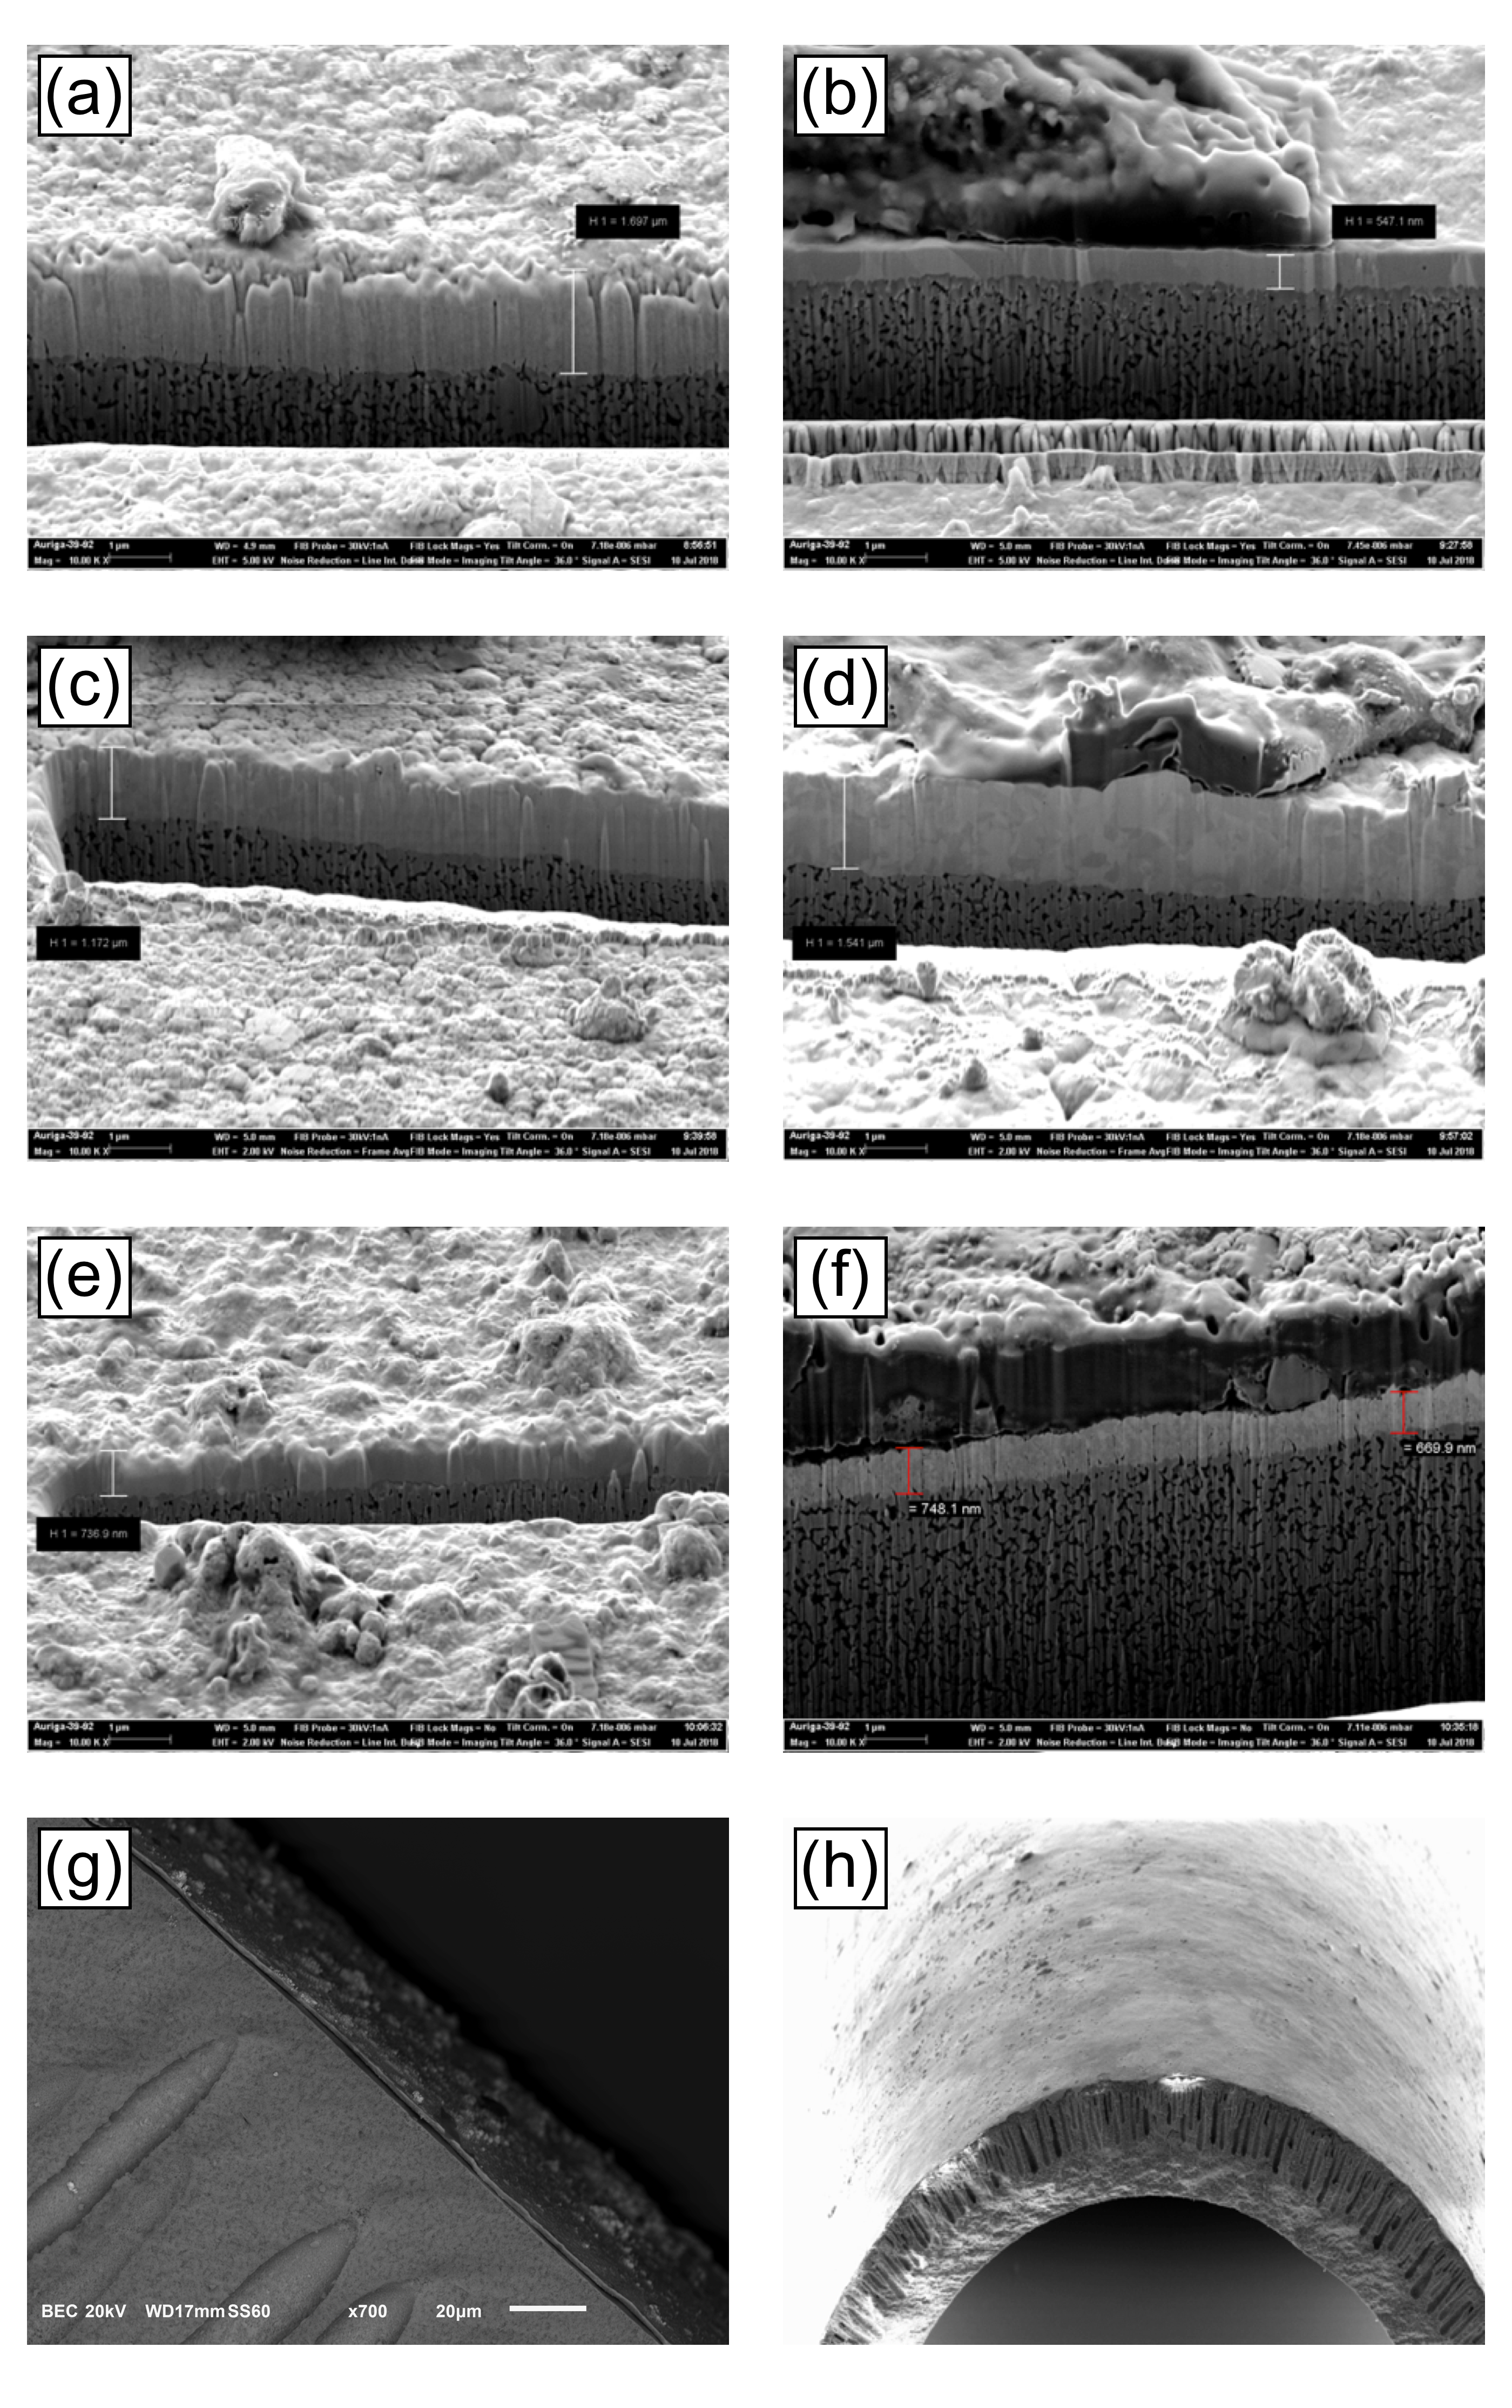
\includegraphics[width=\linewidth, height=0.9\textheight,keepaspectratio]{figures/Semxsect.png}
    \caption{SEM images of fabricated membranes (a) PdCu (fcc) (Sputtering) (b) PdAg (ELP) (c)PdAu (ELP) (d) PdCuZr (Sputtering) (e) PdAgAu (ELP) (f) PdCuAg (ELP) (g) PdCu (bcc) (Sputtering) (h) typical cross section}
    \label{fig:1}
\end{figure}

The surface composition of each membrane was measured by XPS and is shown in Table \ref{results:1}. A wide range of compositions were fabricated. From phase data on the PdCu system \cite{Roa2003, Nayebossadri2013} both varieties of PdCu membranes (bcc phase and fcc phase) were successfully fabricated. In addition to this PdCuZr ternary alloy was fabricated through magnetron sputtering as there is evidence in literature that this alloy composition shows high resistance to impurities and Zr cannot be deposited through electroless plating. \cite{Nayebossadri2013}

\begin{table}[]
    \centering
    \caption{Membrane compositions analysed by EDS and their thickness measured using FIB-SEM}
    \label{results:1}
    \resizebox{\textwidth}{!}{\begin{tabular}{@{}cccccccc@{}}
    \toprule
    \multicolumn{1}{c}{\multirow{2}{*}{Membrane ID}} & \multirow{2}{*}{Manufacturing technique} & \multicolumn{5}{c}{Composition (wt\%) (+- 1\% Relative)} & \multirow{2}{*}{Thickness (um)} \\
    \multicolumn{1}{c}{}                             &                                          & Pd        & Cu        & Ag        & Au        & Zr       &                                 \\ \midrule
    PdCu (Fcc)                                        & Magnetron Sputtering                     & 76.24     & 23.76     & -         & -         & -        & 1.679                           \\
    PdCu (Bcc)                                        & Magnetron Sputtering                     & 43.24     & 56.64     & -         & -         & -        & 1.664                           \\
    PdCuZr                                            & Magnetron Sputtering                     & 72.10     & 14.46     & -         & -         & 13.54    & 1.541                           \\
    PdAg                                              & Electroless Plating                      & 65.55     & -         & 34.45     & -         & -        & 0.573                           \\
    PdAu                                              & Electroless Plating                      & 74.7      & -         & -         & 25.3      & -        & 1.172                           \\
    PdCuAg                                            & Electroless Plating                      & 72.1      & -         & 8.27      & 19.58     & -        & 0.867                           \\
    PdCuAu                                            & Electroless Plating                      & 63.90     & 13.6      & -         & 22.1      & -        & 1.545                           \\
    PdAuAg                                            & Electroless Plating                      & 60        & -         & 11.2      & 28.3      & -        & 0.736                           \\ \bottomrule
    \end{tabular}}
\end{table}

Silver is the most popular dopant for palladium membranes and forms a stable alloy with palladium at concentrations greater than 20 wt\%, with the optimal composition occurring at 23 wt\%. On top of mitigating the effects of hydrogen embrittlement, a $~$60\% increase in permeability is observed when compared to pure Pd membranes. Despite having enhanced permeation properties, PdAg is still susceptible to poisoning, in particular from sulphurous compounds which can form both Pd\textsubscript{4}S and Ag\textsubscript{5}Pd\textsubscript{10}S\textsubscript{5}. A composition of Pd\textsubscript{64.9}Ag\textsubscript{35.1} wt\% was achieved, which, while higher than the desired composition of Pd\textsubscript{77}Ag\textsubscript{23} wt\%, was determined adequate for the purposes of this study.

Copper is another widely studied binary alloy which is known to suppress hydrogen embrittlement. Alloying with copper also has the advantage that it reduces the cost of the membrane by a larger amount than most other metals and through improving the membranes sulphur resistance. The maximum permeability of a palladium copper membrane occurs at the composition Pd\textsubscript{60}Cu\textsubscript{40} wt\% and this is due to the formation of a bcc lattice rather than the fcc lattice commonly seen in pure palladium and most binary alloys. \cite{She2014} Temperature cycling has previously been performed on this alloy composition and it has been found that the bcc crystalline configuration has a higher permeability than the fcc phase. \cite{Dolan2010} This behaviour is due to the increased number of hcp adsorption sites which hydrogen has a slight preference for, and the bcc structure allowing faster diffusion through the bulk of the membrane. \cite{Wilcox2010} Conversely the fcc structure has a higher impurity resistance than the bcc structure, particularly for H\textsubscript{2}S. \cite{She2014, D.T.Hughes1978} Pd\textsubscript{44}Cu\textsubscript{66} and Pd\textsubscript{65.5}Cu\textsubscript{34.5} wt \%  membranes were manufactured using magnetron sputtering which were in the range for bcc and fcc phases respectively.

PdAu alloys see a slight increase in permeability, up to 30\% more than pure Pd \cite{Atsonios2015}, with gold additions up to 20\%, after which the permeability rapidly decreases. While alloying with gold does not improve the permeability much compared to silver or copper, gold alloys show greatly improved sulphur resistance. \cite{Chen2010} The synthesised membrane was found to have the composition  Pd\textsubscript{74.7}Au\textsubscript{25.3} which, while containing a high amount of gold resulting in lower permeation, will have a higher impurity resistance. 

\subsection{Hydrogen permeation}
Table 6 shows the hydrogen permeation through the 9 tested membranes at steady state after 12 hours of operation. As expected, hydrogen permeation flux increases with the elevated temperatures. Moreover, the mass transfer resistance of the substrate will not represent major limitations since its gas transport resistance is negligible compared to that of the dense palladium alloy layer10. Deposited layers were all on the scale of 0.5-2 $\mu$m which from previous research indicates the main rate limiting step in hydrogen permeation being the thickness of the membrane layer. \cite{NathanW.Ockwig2007a} The palladium copper alloy which was in the bcc phase showed the highest hydrogen permeability of all the synthesised membranes which was expected as discussed in \textbf{section 3.1}. The membrane which showed the lowest hydrogen permeability was the PdCuZr membrane, this is likely due to the combined effects of the alloy having an fcc structure, and the alloy having the lowest concentration of palladium compared to the other synthesised membrane, resulting in the lowest number of sites for hydrogen dissociation and subsequent permeation. The PdAu and PdAuAg membranes both showed low permeabilities. Gold as an alloying material traditionally does not show much increase in permeability \cite{Chen2010}  but is instead used to suppress the effects of impurities on the membrane, \cite{Chen2010} which is the main goal of this study. Despite the fact that the commercial membrane is also based on PdAgAu, the membrane manufactured through electroless plating has a lower permeability due to the high gold concentration. It is likely that the concentration of silver in the commercial membrane is closer to 23\%, which is the optimal value for hydrogen permeation, and it’s gold concentration is much lower than the electroless plated membrane. Both PdCuAg and PdCuAu had reasonably high hydrogen permeabilities. While none of these membranes showed a hydrogen permeability as high as the commercial alloy, it should be noted that the commercial membrane had a much larger thickness resulting in a much higher cost and lower flux values than the composite membranes. 

\begin{table}[]
    \centering
    \caption{Pure hydrogen permeability of studied alloy membranes under pure hydrogen at 300\textdegree C and 1 bar pressure differential}
    \label{results:2}
    \begin{tabular}{@{}cc@{}}
        \toprule
        \multicolumn{1}{c}{Membrane ID} & \begin{tabular}[c]{@{}c@{}}Permeability\\ ($mol\:m^{-1} s^{-1} pa^{1/2} \times 10^{-8}$)\end{tabular} \\ \midrule
        PdCu (Fcc)                       & 1.30                                                                                               \\
        PdCu (Bcc)                       & 1.68                                                                                               \\
        PdCuZr                           & 0.14                                                                                               \\
        PdAg                             & 0.94                                                                                               \\
        PdAu                             & 0.33                                                                                               \\
        PdCuAg                           & 1.22                                                                                               \\
        PdCuAu                           & 1.43                                                                                               \\
        PdAuAg                           & 0.19                                                                                               \\
        Commercial (REB)                 & 5.71                                                                                               \\ \bottomrule
        \end{tabular}
\end{table}


\subsection{Impurity reactivity}

\begin{table}[]
\centering
\caption{Permeability results for all membranes under both impurity conditions}
\label{results:3}
\begin{tabular}{@{}cccccl@{}}
\toprule
\multirow{2}{*}{Membrane ID} & \multicolumn{3}{c}{\begin{tabular}[c]{@{}c@{}}Permeability\\ ($mol\:m^{-1} s^{-1} pa^{1/2} \times 10^{-8}$)\end{tabular}} & \multicolumn{2}{c}{\% Drop} \\
                             & Pure H\textsubscript{2}  & Non-Sulphur & Sulphur & Non-sulphur    & Sulphur    \\ \midrule
PdCu (Fcc)                   & 1.30     & 0.22        & 0.185   & 80\%           & 86\%       \\
PdCu (Bcc)                   & 1.68     & 0.721       & 2.47    & 55\%           & 85\%       \\
PdCuZr                       & 0.14     & 0.12        & 0.101   & 12\%           & 26\%       \\
PdAg                         & 0.94     & 0.117       & 0.007   & 88\%           & 92\%       \\
PdAu                         & 0.33     & 0.165       & 0.215   & 51\%           & 35\%       \\
PdCuAg                       & 1.22     & 0.48        & 0.299   & 61\%           & 75\%       \\
PdCuAu                       & 1.43     & 0.789       & 1.07    & 45\%           & 25\%       \\
PdAuAg                       & 0.19     & 0.163       & 0.142   & 16\%           & 27\%       \\ \bottomrule
\end{tabular}
\end{table}

Table \ref{results:3} shows the results of hydrogen permeation under the presence of the two different impurity conditions discussed in \textbf{Table 4 (Gas mixtures table)} compared to the pure hydrogen permeability values shown in Table \ref{results:2}. The permeability data was taken once the flux had reached steady state after 12 hours of operation. For all membranes there was a reduction in permeability when the membranes were exposed to impurities. The magnitude of this reduction compared to the pure hydrogen permeability is used as an indication of the degree of interaction between the membrane and the impurities.  Table \ref{results:4}c shows the composition of each membrane in between each test in order to measure permanent surface reactions and segregation behaviour of the alloys under the chosen impurities. 

\subsubsection{Binary alloys}
In non-sulphur tests the PdAg binary alloy was the worst performing, with the permeability dropping by 88\% of its original value. This was expected as the addition of silver to a palladium system, while effective at increasing the permeability, does not contribute much to impurity resistance. \cite{Peters2016b} This was further supported by the results of the sulphur tests where the permeability dropped by 92\% and composition analysis in Table \ref{results:4} showing that sulphur was present in 42\% of the surface. The PdAg alloy also showed a large degree of segregation behaviour under non-sulphur impurities which likely contributed to the large reduction in flux, with silver concentration increasing to 75\% at the top 10 nm of the sample, resulting in a large drop in permeability. 

Interestingly the PdCu membrane with a composition in the bcc phase showed higher resistance to non-sulphurous impurities than the fcc phase, with the former only experiencing a 55\% drop in permeability compared to an 80\% drop in permeability in the latter. This again seems to be a result of the segregation behaviour of the alloy, with the PdCu alloy in the fcc phase experiencing a large amount of segregation, with the palladium concentration increasing to around 90\% on the retentate side. Conversely the PdCu composition in the BCC phase membrane only changed slightly. The XPS analysis showed that while the reactivity of sulphur on the surface of both copper based binary membranes was of a similar magnitude, the BCC phase had a slightly lower resistance, with 29\% of the surface containing sulphur after exposure to sulphurous impurities as opposed to the 25\% shown by the fcc phase alloy.

The PdAu alloy showed the best impurity resistance out of the binary alloys tested under both impurity conditions, with only a 51\% and 35\% drop in permeability under non-sulphur and sulphur conditions respectively and only a 12\% concentration of sulphur was observed on the surface after XPS analysis. The alloy showed slight segregation of gold away from the permeate surface under non-sulphur impurity conditions likely due to the fact the difference in interaction strength between gold and palladium with the components of the gas mixture varies widely, with many gases preferentially adsorbing on palladium \cite{Gade2011}.

\begin{table}[]
    \centering
    \caption{XPS composition analysis of the palladium alloy membrane surfaces after impurity tests}
    \label{results:4}
    \resizebox{\textwidth}{!}{\begin{tabular}{@{}ccccccccccccccccc@{}}
    \toprule
    \multirow{2}{*}{Membrane ID} & \multicolumn{5}{c}{Pure Hydrogen Exposure} & \multicolumn{5}{c}{Non-Sulphur Exposure} & \multicolumn{6}{c}{Sulphur Exposure} \\
                                 & Pd     & Ag     & Au     & Cu     & Zr     & Pd      & Ag     & Au    & Cu     & Zr   & Pd    & Ag  & Au  & Cu   & Zr & S    \\ \midrule
    PdCu (Fcc)                   & 65.5   & -      & -      & 35.5   & -      & 92.5    & -      & -     & 7.5    & -    & 67.5  & -   & -   & 7.5  & -  & 25   \\
    PdCu (Bcc)                   & 44     & -      & -      & 66     & -      & 54.85   & -      & -     & 45.15  & -    & 40    & -   & -   & 31   & -  & 29   \\
    PdCuZr                       & 63.6   & -      & -      & 22.6   & 13.8   & 64.4    & -      & -     & 27.5   & 8.5  & 54.2  & -   & -   & 27   & 8  & 10.8 \\
    PdAg                         & 65.5   & 34.5   & -      & -      & -      & 25      & 75     & -     & -      & -    & 29    & 29  & -   & -    & -  & 42   \\
    PdAu                         & 75     & -      & 25     & -      & -      & 82.9    & -      & 17.1  & -      & -    & 71    & -   & 16  & -    & -  & 13   \\
    PdCuAg                       & 64.6   & 9.1    & -      & 26.3   & -      & 8.6     & 8.9    & -     & 82.5   & -    & 6     & 5   & -   & 64   & -  & 25   \\
    PdCuAu                       & 63.9   & -      & 22.5   & 13.6   & -      & 84.9    & -      & 1.46  & 13.6   & -    & 65.3  & -   & 1   & 18.5 & -  & 15.2 \\
    PdAuAg                       & 60     & 11.7   & 28.3   & -      & -      & 47.2    & 49.8   & 3     & -      & -    & 52    & 35  & 1   & -    & -  & 12   \\ \bottomrule
    \end{tabular}}
    \end{table}

\subsubsection{Ternary alloys}
Five ternary alloy compositions were tested including the commercial alloy. The commercial alloy had the highest permeability of all ternary alloys with a value of 5.71 mol m\textsuperscript{-1} s\textsuperscript{-1} pa\textsuperscript{-0.5}x10\textsuperscript{-8} under pure hydrogen and 4.28 mol m\textsuperscript{-1} s\textsuperscript{-1} pa\textsuperscript{-0.}5x 10\textsuperscript{-8}  under non-sulphur conditions, a drop in permeability of 25\%. However, the commercial membrane nearly lost all of its permeability under sulphurous conditions. The PdAuAg membrane manufactured through electroless plating performed better under both impurity conditions than the commercial alloy despite being based on the same composition, only seeing a 16\% and 27\% drop in hydrogen permeability under non-sulphur and sulphur conditions respectively compared to a 25\% and 96\% drop shown by the commercial alloy. The high levels of gold likely contributed to the low levels of sulphur on the surface of the electroless plated PdAuAg membrane. These results indicate that the composition of the commercial membrane, while ideal for separation, does not contain enough gold to withstand the levels of sulphur impurities expected for analytical purposes. 

The worst performing ternary alloy was the PdCuAg alloy which showed large permeability drops under all conditions, 61\% under non-sulphur and 75\% under sulphurous conditions. In addition to these, large degrees of segregation were observed under non-sulphur impurities, with the palladium concentration at the surface dropping to 8.5 wt\%, showing that the alloy is not completely stable under the varying conditions expected during analytical purposes.  

Both gold containing ternary alloys, PdAuAg and PdCuAu, performed well under sulphur conditions, with the PdCuAu alloy only reducing in permeability by 25\% and the PdAgAu membrane by 27\%. The PdCuAu membrane however had a stronger interaction with non-sulphur impurities, indicated by the permeability drop of 45\% when exposed to the non-sulphur containing gas sample. This drop is likely due to the segregation of palladium to the surface with the XPS data indicating an increase of palladium to the surface to 84.9 wt\% from 63.9\%. The best performing ternary membrane was the PdCuZr membrane which showed the smallest drop in permeability of only 12\% non-sulphur conditions, and a permeability percentage drop of 26\% under sulphur conditions which on a similar magnitude to that of the gold containing alloys.

\begin{figure}
    \includegraphics[width=\linewidth]{figures/permeabilitychart.png}
    \caption{Permeability data for pure hydrogen, non-sulphur, and sulphur permeation tests}
    \label{permgraph}
  \end{figure}

\subsubsection{Segregation behaviour}
All membranes tested showed some degree of segregation with the two thinnest membrane samples, PdAg (0.573 micron), PdAuAg (0.736  micron) and PdCuAg (0.873 micron) all showing the highest degrees of segregation. While this may still be a property of the alloy compositions it may also indicate that sub-micron palladium alloys layers are unstable and there may be a minimum thickness for alloys, below which the membrane layer is unstable and frequently varies during operation.

\section{Conclusion}
In order to identify a suitable palladium alloy composition for hydrogen impurity enrichment, eight different membrane compositions were manufactured and tested under three different hydrogen conditions against a commercial palladium membrane. Two different measures were used to compare the membrane compositions suitability for hydrogen impurity enrichment, the permeability deviation from the pure hydrogen permeability was used as an initial indicator of interaction between the alloy and impurities, and the surface composition was measured to detect any impurities which had permanently reacted with the membrane. 
The best performing membrane, and therefore the most suitable for hydrogen impurity enrichment was the PdCuZr alloy, which only showed a 12\% and 26\% drop in permeability under non-sulphur, and sulphur conditions, and low levels of sulphur on the surface.  The permeability of this alloy was low, however, surface areas could easily be scaled up to increase the speed of hydrogen enrichment. 

\bibliographystyle{unsrtnat}
\bibliography{library.bib}

\chapter{A hydrogen impurity measurement device for measuring ISO 14687 impurities}

\section{Abstract}
In this chapter a device capable of performing hydrogen impurity enrichment is designed and tested under a number of conditions.

\section{Introduction}

\section{Results and discussion}

\section{Conclusion}
% \bibliographystyle{plainnat}
% \bibliography{library.bib}

\chapter{Conclusion and future work}

\section{Impurity enrichment devices}
\subsection{Further research}
\subsection{Additional use cases}
\subsection{Commercialisation}

\section{Closing remarks}



% \bibliographystyle{plainnat}
% \bibliography{library.bib}

\end{document}